\subsection {Vermessung der Solarzelle POW112D2P}                   % 2.2
    \subsubsection{Aufnehmen der I-U Kennlinie}                         % 2.2 a
        \textbf{Methode}
        \newline
        
        \par Zunächst soll die Solarzelle mit drei unterschiedlichen Lichtquellen bestrahlt werden. Hierbei wird eine Schaltung aufgestellt, bestehend aus einer Diode, welche eine umgekehrte Stromrichtung verhindert, einer Zener-Diode, die die maximale Spannung eingrenzt, und einem Spannungsteiler. Angeschlossen werden die Solarzelle sowie das TI-Board.
        
        \begin{figure}[H]
            $$
            \ctikzset{bipoles/length=1cm}
            \begin{circuitikz}[european] \draw
                (0,0) to[current source, l={\footnotesize $\small Solarzelle$}] (0,4)
                (0,4) to[stroke diode, l={\footnotesize $Diode$}] (2,4)
                (2,0) to[stroke Zener diode, l_={\footnotesize $Zener\ Diode$}] (2,4)
                (0,0) to (2,0)
                (2,4) to (6,4)
                (6,4) to[R, l={\footnotesize $100\ k\Omega$}] (6,2)
                (6,2) to (5,2)
                (5,2) to[capacitor, l_={\footnotesize $100\ nF$}] (5,0)
                (2,0) to (5,0)
                (6,2) to[R, l={\footnotesize $100\ k\Omega$}] (6,0)
                (5,0) to (6,0)
                (6,2) to (8,2)
                (8,2) to[voltmeter, o-o] (8,0)
                (6,0) to (8,0)
                (6,4) to (10,4)
                (10,4) to[R, o-o, l={\footnotesize $Variabler\ Widerstand$}] (10,0)
                (8,0) to (10,0)
                ;
            \end{circuitikz}
            $$
            
            \caption{Benutzter Schaltkreis}
            \label{fig:Schaltkreis}
        \end{figure}
        
        \par Unter gleichbleibenden Bedingungen wurde die Spannung in Abhängigkeit des Widerstandes gemessen, indem Widerstände in Reihe geschaltet wurden. Es wurden in diesem Fall zwölf Widerstände in einem Intervall zwischen 10$\Omega$ bis 5200$\Omega$ verwendet. Mit MatLab lässt sich die Stromstärke aufgrund von I = U/R ermitteln, sodass man sich den Graphen der Stromstärke in Abhängigkeit der Spannung zeichnen lassen kann. (vgl. S.18, \cite{kalman})
        Die Werte der Lichtquellen sind in Tabelle \ref{tab:Werte} abgebildet:
        \begin{table}[htb]
        	\centering
        	\caption{Angaben über Lichtquellen}
        	\label{tab:Werte}
        	\begin{tabular}{ccc}
        		\toprule
        		Art & Leistung & Abstand \\
        		\midrule
        		Halogenlampe & 500W  & 70cm \\
        		Leuchtstoffröhre & 24W  & 13cm \\
        		LED & 40W & 2,5cm \\
        		\bottomrule
        	\end{tabular}
        \end{table}
        
        \vspace{4mm}
        \par Zur graphischen Darstellung wurde folgender Matlab code verwendet:
        
        \begin{figure}[H]
            \lstinputlisting[style=Matlab, firstline=24, lastline=30]{messungen/Aufgabe_2_2/Messungen_2.5cm_40Watt_LED/stromstarke_spannung.m}
            \caption{Matlab code zur graphischen Darstellung der Spannung}
        \end{figure}
        
        
        \vspace{5mm}
        \textbf{Ergebnis}
        \newline
        
        \begin{figure}[H]
            %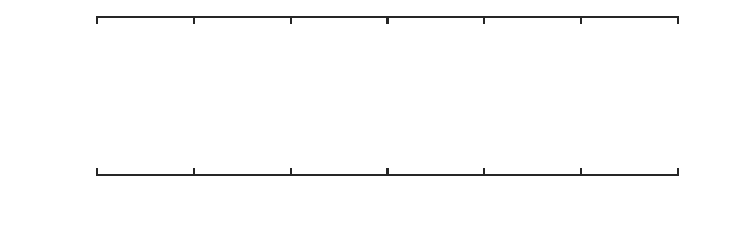
\includegraphics{spannung_halogen}
            \def\svgwidth{\textwidth}
            \input{spannung_halogen.pdf_tex}
            
            \caption{Stromstärke in Abhänigkeit der Spannung bei der Halogenlampe}
        \end{figure}
        
        \begin{figure}[H]
            %\includegraphics{spannung_lsr}
            \def\svgwidth{\textwidth}
            \input{spannung_lsr.pdf_tex}
            
            \caption{Stromstärke in Abhänigkeit der Spannung bei der Leuchtstoffröhre}
        \end{figure}
        
        \begin{figure}[H]
            %\includegraphics{spannung_led}
            \def\svgwidth{\textwidth}
            \input{spannung_led.pdf_tex}
            
            \caption{Stromstärke in Abhänigkeit der Spannung bei der LED}
        \end{figure}

    \subsubsection{Bestimmung des Maximum-Power-Points (MPP)}           % 2.2 b
        \textbf{Methode}
        \newline
        \par Die Leistung hängt von der Spannung sowie der Stromstärke ab aufgrund des Zusammenhanges $P=U*I$. Alternativ gilt wegen $I=U/R$ ebenfalls $P=U^2/R$, welche hier bevorzugt wird, da die Spannung sowie der Widerstand direkte Messwerte sind. Das vorhandene Skript für die Ermittlung der Stromstärke wird um einen Vektor für die Leistung erweitert.
        Der Maximum Power Point (wird nun MPP abgekürzt) bezeichnet nun den Punkt, an dem die Leistung am größten ist. Dieser maximale Wert für die Leistung sowie der dementsprechende Widerstand lassen sich ablesen / von folgendem Matlab code ausgeben:
        
        \begin{figure}[H]
            \lstinputlisting[style=Matlab, firstline=22, lastline=48]{messungen/Aufgabe_2_2/Messungen_2.5cm_40Watt_LED/stromstarke_leistung_spannung.m}
            \caption{Matlab code zur Berechnung der Spannung bzw. Stromstärke und des MPP}
        \end{figure}
        
        \vspace{4mm}
        \textbf{Ergebnis}
        \par Der MPP der Solarzelle unter der Verwendung einer Halogenlampe beträgt ca. 0,0313W und tritt bei 690 Ohm auf. Mit einer Leuchtstoffröhre liegt die maximale Leistung bei ungefähr 0,0075W, welche bei einem Widerstand von 1720 Ohm erreicht wird. Wird hingegen eine LED als Lichtquelle eingesetzt, befindet sich der MPP bei ca. 0,0059W bei einem Widerstand von 2200 Ohm.
        \par Anzumerken ist, dass es sich hierbei nur um einen groben Näherungswert handelt, da lediglich zwölf Messwerte für die Leitung vorliegen. Für eine genauere Bestimmung des MPPs kann mithilfe dieser Werte eine Näherungsfunktion aufgestellt werden, mit dessen Ableitung das Maximum ermittelt werden kann. 
        Diskussion:
        \par Eine weitere Methode zur Bestimmung des MPPs ist über die Spannung und die Stromstärke möglich. So ist die Leistung das Produkt dieser, was auf die I-U-Kennlinie bezogen bedeutet, dass die Leistung den Flächeninhalt unter einem Punkt des Graphen wiederspiegelt. So bezeichnet man den Punkt der Kennlinie als MPP, unter dem die Fläche U*I am größten ist. \par (vgl. S.99, Photovoltaik)
        \par Dieser Zusammenhang wird in dem folgenden Diagramm veranschaulicht.

        \begin{figure}[H]
            \def\svgwidth{\textwidth}
            \input{stromstarke_leistung_spannung_halogen.pdf_tex}
            \caption{Darstellung MPP bei benutzun von Halogenlampe}
        \end{figure}
        
        \begin{figure}[H]
            \def\svgwidth{\textwidth}
            \input{stromstarke_leistung_spannung_lsr.pdf_tex}
            \caption{Darstellung MPP bei benutzun von Leuchtstoffröhre}
        \end{figure}
        
        \begin{figure}[H]
            \def\svgwidth{\textwidth}
            \input{stromstarke_leistung_spannung_led.pdf_tex}
            \caption{Darstellung MPP bei benutzun von LED}
        \end{figure}
        
    \subsubsection{MPP-Anpassung}                                       % 2.2 c
        \textbf{Diskussion}
        \newline
        \par Solarwechselrichter sind dafür zuständig, die von der Solarzelle produzierte Gleichspannung in Wechselspannung umzuwandeln. Für die maximale Leistungsausbeute wird der MPP benötigt(bildet der im Solarwechselrichter enthaltende MPP-Tracker den optimalen Widerstand für den MPP), welcher jedoch unter natürlichen Bedingungen von verschiedenen äußeren Faktoren wie Verschattung, Temperatur oder Lichteinfall abhängt, sodass der MPP stets neu ermittelt werden muss (vgl. S.8f, Diplomarbeit). 
        \par Vernachlässigt wurden Diode/Zehnerdiode, da dort auch Spannung noch abfallen, kleiner Messfehler.
